\chapter{Champs quantiques locaux et équation de Dirac en une dimension}

Nous avons déjà rencontré les champs quantiques à travers leurs quanta, leurs opérateurs de création et d’annihilation, ainsi que le Hamiltonien le plus simple pour des particules non relativistes. Nous allons maintenant mettre ces outils à l’œuvre. Nous verrons d’abord, au lieu de simplement l’affirmer, comment un Hamiltonien local dans l’espace conserve la quantité de mouvement. Puis nous laisserons les produits de champs décrire la diffusion et la désintégration, et observerons comment les applications répétées du Hamiltonien font apparaître les premiers éléments de la théorie perturbative diagrammatique. Ce n’est qu’ensuite que nous aborderons le problème des fermions annoncé. Le point de départ le plus simple n’est pas encore un champ fermionique, mais l’équation de Dirac en une dimension.

\section{Le Hamiltonien de champ, encore une fois}

Écrivons le Hamiltonien d’une espèce de particules non relativistes sous la forme
\begin{equation}
H_0=\int dx\,
\psi^\dagger(x)
\left[-\frac{\partial_x^2}{2m}+V(x)\right]
\psi(x).
\label{eq:l9-nonrel-hamiltonian}
\end{equation}
La notation semble unidimensionnelle, mais rien dans l’argument initial ne dépend de cette restriction : en trois dimensions, \(x\) peut désigner le vecteur \(\mathbf{x}\), \(dx\) peut désigner \(d^3x\), et \(-\partial_x^2\) peut désigner \(-\nabla^2\).

L’opérateur \(\psi^\dagger(x)\) crée une particule en \(x\), tandis que \(\psi(x)\) en annihile une à cet endroit. Leur produit normalement ordonné
\begin{equation}
n(x)=\psi^\dagger(x)\psi(x)
\end{equation}
est la densité locale de particules. Le terme de potentiel s’écrit donc
\begin{equation}
H_V=\int dx\,V(x)n(x).
\end{equation}
C’est exactement ce que nous écririons pour un gaz classique : compter les particules près de \(x\), attribuer à chacune l’énergie potentielle \(V(x)\), puis sommer sur tout l’espace. À ce stade, les particules n’interagissent pas entre elles. Elles peuvent réagir à un potentiel externe imposé, mais le Hamiltonien est par ailleurs une somme d’énergies indépendantes pour chaque particule.

Il est utile de simplifier, puis de revenir sur cette simplification. Prenons un potentiel constant, \(V(x)=V_0\). Un potentiel constant n’exerce aucune force, mais sa signification en tant qu’opérateur est transparente :
\begin{equation}
\begin{aligned}
H_V&=V_0\int dx\,\psi^\dagger(x)\psi(x)=V_0N,\\
N&=\int dx\,n(x).
\end{aligned}
\end{equation}
Il attribue à chaque particule la même énergie additive. Pour conserver l’énergie de repos dans une description non relativiste, choisissons \(V_0=mc^2\). Le terme compte alors une énergie de repos par particule. Nous gardons cette constante par ailleurs peu intéressante parce qu’elle préserve l’invariance par translation et rend visible l’opération de comptage des particules.

\section{Le Hamiltonien comme règle d’évolution}

Que signifie l’affirmation selon laquelle la quantité de mouvement est conservée ? Il faut formuler la réponse en termes de l’action du Hamiltonien. Pour éviter d’employer \(\psi\) à la fois pour un opérateur de champ, une fonction d’onde à une particule et un état à plusieurs corps, notons l’état à plusieurs corps \(\lvert\Phi(t)\rangle\). Sur un court intervalle \(\epsilon\),
\begin{equation}
\lvert\Phi(t+\epsilon)\rangle
=\left(1-i\epsilon H+O(\epsilon^2)\right)
\lvert\Phi(t)\rangle,
\label{eq:l9-short-update}
\end{equation}
où \(\hbar=1\). Le premier terme est l’état inchangé ; la première correction est engendrée par \(H\). La répétition de cette évolution donne l’équation de Schr\"odinger.

La conservation de la quantité de mouvement prend maintenant un sens concret. Si l’état initial possède une quantité de mouvement totale bien définie \(P\), alors \(H\lvert\Phi\rangle\) doit avoir cette même quantité de mouvement totale. D’autres propriétés peuvent changer, et les particules individuelles peuvent échanger de la quantité de mouvement, mais le Hamiltonien ne peut pas faire passer l’état dans un secteur où la quantité de mouvement totale \(P\) est différente. Nous pouvons le vérifier directement en réécrivant le Hamiltonien dans la base des impulsions.

\section{L’intégrale spatiale comme delta de Dirac en impulsion}

Choisissons la convention de Fourier
\begin{align}
\psi(x)&=\int\frac{dp}{\sqrt{2\pi}}\,a(p)e^{ipx},\\
\psi^\dagger(x)&=\int\frac{dq}{\sqrt{2\pi}}\,a^\dagger(q)e^{-iqx}.
\label{eq:l9-field-fourier}
\end{align}
L’opérateur \(a(p)\) annihile une particule d’impulsion \(p\).
L’opérateur \(a^\dagger(q)\) en crée une d’impulsion \(q\). Il est essentiel d’utiliser des lettres différentes : les deux impulsions sont intégrées indépendamment jusqu’à ce que l’intégrale spatiale les relie.

Commençons par le terme de comptage :
\begin{align}
N
&=\int dx\,\psi^\dagger(x)\psi(x)\\
&=\int\frac{dp\,dq}{2\pi}\,
a^\dagger(q)a(p)
\int dx\,e^{i(p-q)x}.
\end{align}
L’intégrale restante est
\begin{equation}
\int dx\,e^{i(p-q)x}=2\pi\delta(p-q).
\end{equation}
Pour \(p\ne q\), la phase oscille et les contributions positives et négatives s’annulent. Pour \(p=q\), elle n’oscille pas du tout. La distribution delta de Dirac est l’objet précis qui réunit ces deux faits. Par conséquent,
\begin{align}
N
&=\int dp\,dq\,a^\dagger(q)a(p)\delta(p-q)\\
&=\int dp\,a^\dagger(p)a(p).
\label{eq:l9-number-momentum}
\end{align}
L’opérateur enlève une particule d’impulsion \(p\) et en remet une d’exactement la même impulsion. L’élément décisif était l’intégrale sur \(x\) : elle a produit le delta qui impose l’égalité entre les impulsions entrante et sortante.

\begin{classroomqa}
\lecturetimestamp{00:17:02}
\audiencequestion{Que devient l’infini qui apparaît lorsque \(p=q\) ?}
\lecturerresponse{Une fonction delta ne s’évalue pas en considérant sa hauteur. C’est une distribution définie par intégration : \(\int dk\,\delta(k)f(k)=f(0)\). L’expression ``infiniment haute et infiniment étroite'' rappelle seulement que son poids intégré vaut un. Ici, elle nous indique de poser \(p-q=0\), et il ne reste aucun résultat infini.}
\end{classroomqa}

Le même mécanisme s’applique à un monôme local bien plus général. Supposons qu’un terme contienne plusieurs champs d’annihilation et plusieurs champs de création, appartenant éventuellement à différentes espèces, tous évalués au même point et intégrés sur ce point :
\begin{equation}
\int dx\,
\prod_{r=1}^{n} \psi_{i_r}^\dagger(x)
\prod_{s=1}^{m} \psi_{j_s}(x).
\end{equation}
Notons \(p_s\) les impulsions des particules annihilées et \(q_r\) celles des particules créées. Le développement de Fourier donne
\begin{equation}
\int dx\,
e^{i(\sum_s p_s-\sum_r q_r)x}
=2\pi\,
\delta\!\left(\sum_s p_s-\sum_r q_r\right).
\label{eq:l9-total-momentum-delta}
\end{equation}
Le résultat n’apparie pas \(p_1\) avec \(q_1\), \(p_2\) avec \(q_2\), et ainsi de suite. Il impose seulement
\begin{equation}
\sum_{\mathrm{annihilated}}p
=
\sum_{\mathrm{created}}q.
\end{equation}
C’est exactement la règle requise pour une interaction : les impulsions individuelles peuvent changer, mais pas la quantité de mouvement totale. L’énoncé plus profond est celui de l’invariance par translation. Une densité locale intégrée avec le même poids en chaque point ne privilégie aucune origine, et sa transformée de Fourier contient le delta de Dirac correspondant qui conserve la quantité de mouvement.

\begin{classroomqa}
\lecturetimestamp{00:23:04}
\audiencequestion{Le terme de Hamiltonien proposé est-il vraiment un produit de tous ces opérateurs de champ ? Pourquoi écrirait-on un tel produit ?}
\lecturerresponse{Oui. Le produit précise quelles particules sont enlevées et lesquelles sont créées en un même point. Sa motivation physique viendra des processus de diffusion ou de désintégration observés ; l’argument sur la quantité de mouvement est établi d’abord afin que ces interactions puissent être interprétées immédiatement.}
\end{classroomqa}

\section{Énergie cinétique dans l’espace des impulsions et dans l’espace des positions}

Appliquons maintenant le même procédé au terme dérivé. La dérivée agit sur l’onde plane :
\begin{equation}
-\partial_x^2 e^{ipx}=p^2e^{ipx}.
\end{equation}
Par conséquent,
\begin{align}
H_{\mathrm{kin}}
&=\int dx\,\psi^\dagger(x)
\left(-\frac{\partial_x^2}{2m}\right)\psi(x)\\
&=\int dp\,\frac{p^2}{2m}\,a^\dagger(p)a(p).
\label{eq:l9-kinetic-momentum}
\end{align}
Là encore, l’intégrale spatiale impose l’égalité des impulsions entrante et sortante. Le nouveau facteur \(p^2/2m\) pondère simplement le nombre de particules dans chaque mode d’impulsion par l’énergie cinétique de ce mode.

\begin{classroomqa}
\lecturetimestamp{00:24:46}
\audiencequestion{La dérivée seconde de l’onde plane ne devrait-elle pas donner un signe moins ?}
\lecturerresponse{Oui, \(\partial_x^2e^{ipx}=-p^2e^{ipx}\). Le Hamiltonien contient déjà le signe moins compensateur, de sorte que \(-\partial_x^2\) a pour valeur propre positive \(p^2\).}
\end{classroomqa}

\begin{classroomqa}
\lecturetimestamp{00:27:20}
\audiencequestion{L’énergie cinétique est-elle conservée uniquement lorsque le potentiel est constant ?}
\lecturerresponse{Oui. En l’absence de potentiel dépendant de la position, il n’y a pas de force et l’énergie cinétique est conservée séparément. Dans un potentiel externe non constant, les énergies cinétique et potentielle peuvent s’échanger, tandis que le Hamiltonien total reste conservé s’il ne dépend pas explicitement du temps.}
\end{classroomqa}

\begin{classroomqa}
\lecturetimestamp{00:27:42}
\audiencequestion{Quel est le rôle de \(\psi^\dagger\psi\) dans le Hamiltonien cinétique en espace des impulsions ?}
\lecturerresponse{C’est l’opérateur de comptage. Le produit de modes \(a^\dagger(p)a(p)\) compte les particules d’impulsion \(p\), et le facteur \(p^2/2m\) attribue à chacune l’énergie cinétique appropriée.}
\end{classroomqa}

On peut aussi établir la positivité d’une seconde manière. Une intégration par parties et l’omission du terme de bord donnent
\begin{align}
\int dx\,\psi^\dagger(-\partial_x^2)\psi
&=\int dx\,(\partial_x\psi^\dagger)(\partial_x\psi).
\label{eq:l9-positive-kinetic}
\end{align}
Pour des champs qui s’annulent suffisamment à l’infini, ou avec des conditions aux limites périodiques, la contribution de bord est nulle. Le résultat prend la forme d’un carré de module et est donc non négatif. Il met aussi en évidence un motif courant en théorie des champs : l’énergie contient des carrés de dérivées spatiales des champs.

\section{Une interaction locale de contact}

Donnons maintenant un rôle physique aux produits de champs. Considérons deux espèces, que nous appellerons électron et proton uniquement pour rendre le tableau familier. Pour l’instant, il s’agit délibérément de particules fictives : toutes deux sont décrites par des opérateurs bosoniques, et leur véritable interaction coulombienne est omise. Leur Hamiltonien libre est
\begin{equation}
H_0=\int dx\left[
\psi_e^\dagger\left(-\frac{\partial_x^2}{2m_e}\right)\psi_e
+
\psi_p^\dagger\left(-\frac{\partial_x^2}{2m_p}\right)\psi_p
\right].
\end{equation}
Ajoutons l’interaction modèle
\begin{equation}
H_{\mathrm{contact}}
=g\int dx\,
\psi_e^\dagger(x)\psi_p^\dagger(x)
\psi_e(x)\psi_p(x).
\label{eq:l9-contact}
\end{equation}
Lisons-la de droite à gauche. Elle repère un électron et un proton au même point \(x\), les annihile, puis recrée les deux à cet endroit. Si les deux particules ne sont pas ensemble, ce terme local est nul. Si leurs lignes d’univers se rencontrent, il peut modifier leurs impulsions individuelles tout en préservant la quantité de mouvement totale. Il agit donc comme un potentiel de diffusion idéalisé de portée nulle.

\begin{figure}[htbp]\centering
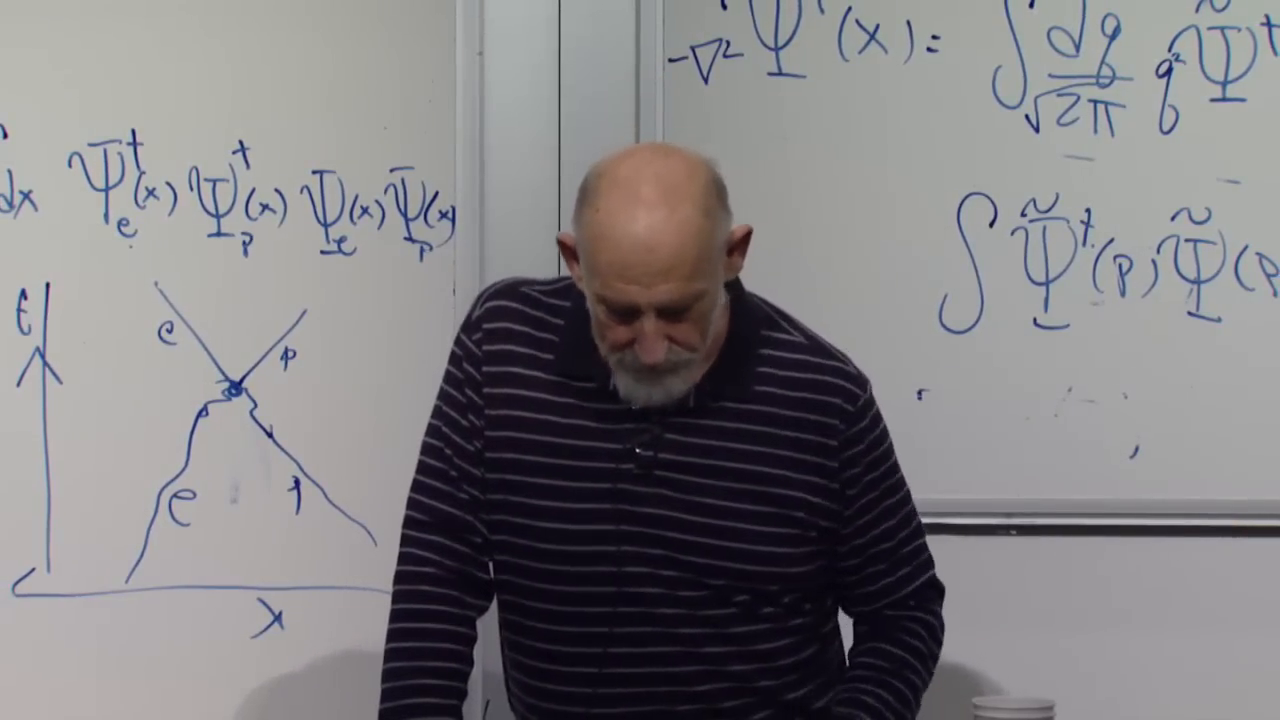
\includegraphics[width=0.94\linewidth]{lecture_09_frame_02.png}\caption{L’interaction de contact au tableau. Les quatre opérateurs de champ locaux figurent au-dessus du croquis d’espace-temps ; le point de rencontre est le seul endroit où agit l’interaction idéalisée.}\lectureframe{00:35:36}\end{figure}

\begin{figure}[htbp]\centering
\begin{tikzpicture}[x=1.2cm,y=1.0cm,>=Latex]
\draw[->] (-3.0,0) -- (3.0,0) node[right] {$x$};
\draw[->] (0,-0.2) -- (0,4.2) node[above] {$t$};
\coordinate (v) at (0,2.0);
\fill (v) circle (1.8pt);
\draw[thick,->] (-2.2,0.4) -- (v);
\draw[thick,->] (2.0,0.4) -- (v);
\draw[thick,->] (v) -- (-1.6,3.7);
\draw[thick,->] (v) -- (2.2,3.7);
\node[left] at (-1.65,0.7) {$e$};
\node[right] at (1.55,0.7) {$p$};
\node[left] at (-1.15,3.3) {$e$};
\node[right] at (1.65,3.3) {$p$};
\node[right] at (0.12,2.05) {$g$};
\end{tikzpicture}\caption{Reconstitution épurée du schéma de diffusion locale. Le sommet est une notation abrégée pour l’opérateur de l’équation ~\eqref{eq:l9-contact}, et non une loi classique de collision.}\end{figure}

Les électrons et les protons réels interagissent à distance par le potentiel coulombien. Le modèle de contact n’est qu’un premier pas, très limité : si l’expérience montrait que deux espèces ne diffusent que lorsqu’elles se recouvrent, l’équation ~\eqref{eq:l9-contact} serait le genre de terme que nous ajouterions au Hamiltonien.

\begin{classroomqa}
\lecturetimestamp{00:35:40}
\audiencequestion{Pourquoi cet opérateur de diffusion fait-il partie du Hamiltonien si l’énergie ne change pas ?}
\lecturerresponse{Le Hamiltonien est à la fois l’opérateur énergie et le générateur de l’évolution de l’état. Une énergie potentielle entre les deux particules produit de la diffusion au cours de l’évolution temporelle. La conservation de l’énergie totale ne signifie pas que l’état, ou les impulsions individuelles des particules, reste inchangé.}
\end{classroomqa}

Cela donne une règle pratique. Il faut d’abord apprendre par l’expérience quels processus locaux les particules peuvent subir. On encode ensuite ces processus dans l’opérateur qui fait évoluer l’état. Les produits de champs ne sont pas une algèbre décorative : leurs facteurs avec ou sans dagger précisent quelles espèces apparaissent et disparaissent.

\section{Désintégration, processus inverse et hermiticité}

Supposons qu’une chambre à bulles révèle la trace d’une espèce \(A\) qui se termine en un point d’où émergent les traces \(B\) et \(C\). Le processus local est
\begin{equation}
A\longrightarrow B+C.
\end{equation}
L’opérateur qui le réalise est
\begin{equation}
V=g\int dx\,
\psi_B^\dagger(x)\psi_C^\dagger(x)\psi_A(x).
\label{eq:l9-decay-half}
\end{equation}
Le champ d’annihilation enlève \(A\) ; les deux champs de création produisent \(B\) et \(C\) au même point. L’intégration avec un poids identique sur chaque \(x\) exprime l’invariance par translation spatiale et fournit immédiatement
\begin{equation}
p_A=p_B+p_C.
\end{equation}

Un Hamiltonien doit être hermitien. C’est ce qui rend \(e^{-itH}\) unitaire et préserve la probabilité totale. L’équation ~\eqref{eq:l9-decay-half} n’est pas hermitienne à elle seule ; nous devons donc ajouter son adjoint :
\begin{equation}
H_{\mathrm{int}}
=\int dx\left[
g\,\psi_B^\dagger\psi_C^\dagger\psi_A
+g^*\,\psi_A^\dagger\psi_C\psi_B
\right](x).
\label{eq:l9-hermitian-vertex}
\end{equation}
Pour un couplage réel \(g\), les deux coefficients sont identiques. La conjugaison hermitienne inverse l’ordre des opérateurs tout en échangeant les champs avec dagger et sans dagger. Dans ce modèle fictif bosonique, les champs d’espèces distinctes commutent, de sorte que cette inversion n’entraîne aucune difficulté supplémentaire.

Le second terme réalise le processus inverse,
\begin{equation}
B+C\longrightarrow A.
\end{equation}
Ainsi, un Hamiltonien fermé et unitaire qui permet la désintégration contient aussi l’amplitude de recombinaison. Cela ne garantit pas que les deux sens se produisent pour tout choix de moments extérieurs ; les lois de conservation de l’énergie et d’autres grandeurs peuvent rendre un sens inaccessible cinématiquement. Cela signifie que l’opérateur et son adjoint font tous deux partie de la dynamique.

\begin{classroomqa}
\lecturetimestamp{00:42:48}
\audiencequestion{Peut-il y avoir une exception à la règle selon laquelle le processus inverse est lui aussi permis ?}
\lecturerresponse{Pas au niveau d’un Hamiltonien hermitien pour un système fermé : l’interaction adjointe est nécessaire. Une réaction inverse particulière peut néanmoins être interdite par la cinématique ou par un autre nombre quantique conservé, mais l’élément de matrice conjugué est présent.}
\end{classroomqa}

Le nombre \(g\) est la constante de couplage. Si \(g\) est petit, les particules qui se rencontrent interagissent faiblement ; s’il est grand, l’amplitude de transition est plus élevée. Les couplages sont généralement des paramètres mesurés expérimentalement, bien que des symétries puissent relier plusieurs couplages apparemment différents.

La même grammaire permet de traiter des réactions plus élaborées. Dans la désintégration bêta,
\begin{equation}
n\longrightarrow p+e^-+\bar\nu_e,
\end{equation}
un terme local schématique contient quatre champs : l’un annihile le neutron et trois créent le proton, l’électron et l’antineutrino électronique, avec le processus hermitien conjugué. Cela suffit à montrer comment un petit nombre de monômes d’opérateurs commence à définir une théorie quantique des champs.

\section{Pourquoi le carré du Hamiltonien est important}

La formule à court terme \eqref{eq:l9-short-update} ne conservait que le premier ordre en \(\epsilon\). Le développement complet est
\begin{equation}
e^{-i\epsilon H}
=1-i\epsilon H-\frac{\epsilon^2}{2}H^2
+\frac{i\epsilon^3}{3!}H^3+\cdots.
\label{eq:l9-exponential}
\end{equation}
Au deuxième ordre, le Hamiltonien agit deux fois. C’est l’origine algébrique des premiers schémas représentant des processus composés.

Pour le sommet \(A\leftrightarrow B+C\), une action peut combiner \(B+C\) en \(A\), puis une seconde peut décomposer cet \(A\) de nouveau en \(B+C\) :
\begin{equation}
B+C\longrightarrow A\longrightarrow B+C.
\label{eq:l9-bc-scattering}
\end{equation}
La contribution nette est une amplitude de diffusion \(B+C\to B+C\). L’état intermédiaire \(A\) ne représente pas un événement observé supplémentaire ; il désigne l’état sur lequel on somme entre deux actions de l’interaction.

\begin{classroomqa}
\lecturetimestamp{00:49:54}
\audiencequestion{Dans le produit du deuxième ordre écrit au tableau, le champ \(C\) devrait-il porter un dagger ?}
\lecturerresponse{Oui, l’ordre des opérateurs doit correspondre à la séquence indiquée. Le premier sommet annihile \(B\) et \(C\) et crée \(A\) ; le second annihile \(A\) et recrée \(B\) et \(C\). L’écriture correcte des daggers correspondants rétablit cette interprétation.}
\end{classroomqa}

\begin{figure}[htbp]\centering
\includegraphics[width=0.94\linewidth]{lecture_09_frame_05.png}\caption{Les deux orientations du sommet élémentaire \(A\leftrightarrow B+C\) dessinées au tableau. Leur juxtaposition est la notation visuelle abrégée du processus du deuxième ordre de l’équation ~\eqref{eq:l9-bc-scattering}.}\lectureframe{00:48:56}\end{figure}

Ajoutons maintenant une particule spectatrice \(B\). Une action permet à \(A\) d’émettre \(C\) et de devenir \(B\) ; lors d’une action ultérieure, cet \(C\) se combine à l’\(B\) initial pour former \(A\). Les particules extérieures sont de nouveau \(A+B\), mais leurs impulsions peuvent changer. Nous décrivons cela comme une diffusion \(A\) et \(B\) par échange de \(C\).

\begin{figure}[htbp]\centering
\includegraphics[width=0.94\linewidth]{lecture_09_frame_06.png}\caption{Le mécanisme d’échange au tableau. Le diagramme de droite relie deux sommets élémentaires par une ligne interne de \(C\), tandis que les particules externes \(A\) et \(B\) diffusent.}\lectureframe{00:51:22}\end{figure}

\begin{figure}[htbp]\centering
\begin{tikzpicture}[x=1.1cm,y=1cm,>=Latex]
\draw[->] (-3.7,-0.2) -- (-3.7,4.2) node[above] {$t$};
\coordinate (v1) at (-0.9,1.25);
\coordinate (v2) at (0.9,2.95);
\fill (v1) circle (1.7pt);
\fill (v2) circle (1.7pt);
\draw[thick,->] (-2.6,0.2) -- (v1) node[midway,below left] {$A$};
\draw[thick,->] (2.6,0.2) -- (v2) node[midway,below right] {$B$};
\draw[thick,->] (v1) -- (-2.4,4.0) node[midway,left] {$B$};
\draw[thick,->] (v2) -- (2.5,4.0) node[midway,right] {$A$};
\draw[thick,->,dashed] (v1) -- (v2) node[midway,above left] {$C$};
\node[below] at (0,-0.05) {$A+B\rightarrow A+B$};
\end{tikzpicture}\caption{Reconstitution épurée de l’échange de \(C\). Chaque point apporte un facteur \(g\) ; ce terme du deuxième ordre est donc proportionnel à \(g^2\).}\end{figure}

Chaque point d’interaction locale est appelé un sommet. Chaque sommet apporte un facteur égal à son couplage ; une contribution à deux sommets comporte donc \(g^2\), une contribution à trois sommets \(g^3\), et ainsi de suite. Un seul terme du Hamiltonien relie ainsi toute une famille de réactions. Cette économie explique en partie la puissance de la théorie quantique des champs : un petit nombre d’interactions locales organise une quantité considérable de données de diffusion.

\begin{classroomqa}
\lecturetimestamp{00:53:14}
\audiencequestion{Comment appelle-t-on le processus \(A\to B+C\to A\) ?}
\lecturerresponse{C’est une contribution à l’auto-énergie. Un \(A\) mesuré n’est pas simplement l’état de base nu à une particule ; l’état en interaction possède aussi une amplitude pour des composantes \(B+C\) voisines. La diffusion sur cet état peut révéler cette structure habillée.}
\end{classroomqa}

L’électrodynamique quantique en fournit l’exemple familier. Un sommet local électron--photon peut annihiler un électron, recréer un électron et créer un photon. Au deuxième ordre, l’électron peut émettre un photon puis le réabsorber. On est tenté d’en faire le récit comme d’un petit film, mais son sens rigoureux est celui d’un terme du développement perturbatif. L’électron physique est un état habillé qui comporte des composantes contenant des photons.

L’estimation donnée en cours, selon laquelle cette composante est ``d’environ un pour cent'', donne une idée de l’échelle fixée par la constante de structure fine, \(\alpha_{\mathrm{em}}\simeq 1/137\). La probabilité précise d’une composante de Fock avec photon dépend de la résolution en énergie et de la définition de l’état en interaction ; ce n’est pas une propriété universelle de l’électron isolé, égale à un pour cent. L’énoncé robuste est que l’interaction modifie la structure mesurable de l’électron.

\section{Ce qu’un diagramme dit et ne dit pas}

Les diagrammes sont une notation abrégée, utile au calcul, pour les puissances du Hamiltonien d’interaction. Ils ne constituent pas des histoires classiques fiables dans lesquelles une particule accomplirait certainement un événement puis un autre. Chercher à déterminer si une alternative intermédiaire ``s’est réellement produite'' modifie l’expérience et détruit la somme cohérente, comme dans une expérience d’interférence quantique ordinaire.

\begin{classroomqa}
\lecturetimestamp{00:56:52}
\audiencequestion{L’énergie et la quantité de mouvement sont-elles toutes deux conservées au premier sommet ?}
\lecturerresponse{Dans la construction hamiltonienne à temps égal effectuée ici, l’intégrale spatiale produit immédiatement un delta de Dirac en impulsion. Aucune intégrale temporelle n’a encore produit de delta en énergie pour cette insertion isolée. L’amplitude de diffusion complète, invariante par translation temporelle, conserve l’énergie totale, tandis que les lignes intermédiaires n’ont pas nécessairement à satisfaire la relation de masse des particules observées. Dans le langage des diagrammes covariants, le quadri-moment est conservé à chaque sommet, mais les particules internes peuvent être hors couche de masse.}
\end{classroomqa}

L’énergie apparemment manquante dans une représentation naïve du sommet rappelle une fois de plus qu’il ne faut pas négliger l’énergie d’interaction. Le Hamiltonien total ne se réduit pas à la somme des énergies des particules libres. En cas de doute, revenons à l’équation ~\eqref{eq:l9-exponential} : le schéma représente un terme du développement de l’évolution unitaire dans le temps. La théorie complète des diagrammes de Feynman fournit un ordre temporel systématique, des propagateurs, des intégrales et des facteurs de symétrie, mais les bases physiques sont déjà là.

Une question plus développée pousse à interpréter le diagramme trop littéralement en comparant le photon émis au champ électrique entourant un électron en mouvement lent.

\begin{classroomqa}
\lecturetimestamp{00:58:26}
\audiencequestion{Le champ électrique de l’électron à distance est-il littéralement produit par des photons rayonnés ? Quel est le lien avec les interférences et l’effet Aharon--Bohm ?}
\lecturerresponse{Un champ statique ou un champ d’induction n’est pas un flux de photons réels rayonnés. L’électrodynamique quantique décrit à la fois le rayonnement et l’habillage électromagnétique de l’électron à l’aide du même champ, mais les états quantiques et les conditions cinématiques correspondants diffèrent. Pour un électron ultrarelativiste, certaines composantes du champ peuvent utilement être assimilées à un flux de photons presque réels ; pour un électron lent, une trajectoire littérale de photon est un modèle inadéquat. L’interférence à deux fentes et l’effet Aharon--Bohm sont eux aussi des phénomènes de champ non classiques, mais ils ne transforment pas ce diagramme d’auto-énergie en film mécanique.}
\end{classroomqa}

\begin{classroomqa}
\lecturetimestamp{01:01:28}
\audiencequestion{Pourquoi exactement un modèle classique du diagramme échoue-t-il ?}
\lecturerresponse{Parce que le calcul additionne de manière cohérente les amplitudes associées à toutes les alternatives intermédiaires permises. L’expérience rend ces schémas intuitifs, mais leur contenu littéral ne dépasse jamais le développement en opérateurs qui les définit. Ils constituent une façon compacte de calculer \(H^2,H^3,\ldots\), et non le compte rendu d’événements intermédiaires observés.}
\end{classroomqa}

\begin{classroomqa}
\lecturetimestamp{01:03:04}
\audiencequestion{L’interaction coulombienne ordinaire peut-elle émerger comme limite classique de l’échange de photons ?}
\lecturerresponse{Oui. Le calcul de l’amplitude appropriée médiée par un photon, suivi de la limite statique non relativiste, donne le potentiel coulombien. La dérivation est plus technique que le présent aperçu des opérateurs ; elle ne doit toujours pas être interprétée comme si un photon sautait littéralement d’une particule classique à une autre.}
\end{classroomqa}

\begin{classroomqa}
\lecturetimestamp{01:03:44}
\audiencequestion{Les constantes de couplage se calculent-elles à partir des produits de champs ?}
\lecturerresponse{Leurs valeurs numériques sont généralement des données expérimentales. Une symétrie peut les contraindre ou relier des couplages qui seraient autrement indépendants. Lorsqu’une telle relation prédit les intensités relatives de réactions distinctes et que l’expérience la confirme, cet accord est particulièrement instructif.}
\end{classroomqa}

\begin{classroomqa}
\lecturetimestamp{01:04:48}
\audiencequestion{Quel est le rôle d’une symétrie accidentelle par rapport à celui d’une symétrie de jauge ?}
\lecturerresponse{Une symétrie de jauge contraint directement la structure permise et les relations entre les couplages. Une symétrie accidentelle n’est pas imposée au niveau fondamental, mais émerge parce que toutes les interactions permises d’ordre inférieur la respectent par hasard. Elle peut néanmoins avoir des conséquences importantes, même si son origine et sa robustesse diffèrent de celles d’une symétrie de jauge.}
\end{classroomqa}

C’est tout pour l’instant sur la théorie non relativiste des champs. Nous avions promis d’aborder les fermions. Au lieu de les quantifier immédiatement en seconde quantification, nous allons d’abord comprendre l’équation relativiste à une particule que leurs opérateurs de champ doivent satisfaire.

\section{Pourquoi l’électron exige une description relativiste}

Commençons par une dimension spatiale. Ce n’est pas une restriction réaliste, mais elle élimine la complexité géométrique du spin en trois dimensions tout en préservant l’algèbre essentielle. L’électron est assez léger pour que les effets relativistes comptent même dans les atomes. Dans l’hydrogène, sa vitesse caractéristique est de l’ordre de
\begin{equation}
v\sim\alpha_{\mathrm{em}}c\approx 0.007c,
\end{equation}
soit environ un pour cent de la vitesse de la lumière. Pour les électrons internes d’un atome lourd, l’ordre de grandeur devient \(v\sim Z\alpha_{\mathrm{em}}c\), et les corrections relativistes peuvent donc être importantes. Que la curiosité historique ou la précision atomique ait fourni la motivation décisive, une équation de type Schr\"odinger relativiste est physiquement nécessaire.

La méthode habituelle de quantification part de la relation classique entre l’énergie et la quantité de mouvement. Dans le cas non relativiste,
\begin{equation}
E=\frac{p^2}{2m},
\end{equation}
et les substitutions
\begin{equation}
E\mapsto i\partial_t,
\qquad
p\mapsto-i\partial_x
\end{equation}
donnent
\begin{equation}
i\partial_t\varphi(x,t)
=-\frac{1}{2m}\partial_x^2\varphi(x,t).
\end{equation}

La relativité donne plutôt, avec \(c=1\),
\begin{equation}
E^2=p^2+m^2.
\label{eq:l9-rel-dispersion}
\end{equation}

\begin{figure}[htbp]\centering
\includegraphics[width=0.94\linewidth]{lecture_09_frame_07.png}\caption{Le passage au tableau de \(E=p^2/2m\) à la relation relativiste \(E^2=p^2+m^2\), avec \(c=1\).}\lectureframe{01:10:30}\end{figure}

Appliquer les substitutions à la relation au carré donne
\begin{equation}
-\partial_t^2\varphi
=\left(-\partial_x^2+m^2\right)\varphi,
\label{eq:l9-klein-gordon}
\end{equation}
ou, de manière équivalente,
\begin{equation}
\left(\partial_t^2-\partial_x^2+m^2\right)\varphi=0.
\end{equation}
C’est l’équation de Klein--Gordon. C’est une équation relativiste de champ parfaitement valable, en particulier pour les champs de spin nul. Mais l’équation recherchée pour l’électron doit être du premier ordre en temps,
\begin{equation}
i\partial_t\Psi=H\Psi,
\end{equation}
afin que \(H\) lui-même, et pas seulement \(H^2\), engendre l’évolution.

On pourrait formellement choisir
\begin{equation}
H=\sqrt{-\partial_x^2+m^2}.
\end{equation}
La racine carrée se définit sans difficulté dans l’espace des impulsions, où elle correspond à une multiplication par \(\sqrt{p^2+m^2}\), mais dans l’espace des positions, c’est un opérateur pseudo-différentiel non local. Il est mathématiquement bien défini, mais peu adapté à l’équation locale que nous cherchons. Repartons donc de zéro.

\section{Une onde sans masse se propageant vers la droite}

Considérons d’abord une particule sans masse se déplaçant vers la droite. Son énergie et son impulsion positives vérifient
\begin{equation}
E=p
\qquad (c=1).
\end{equation}
La quantification donne
\begin{equation}
i\partial_t\psi=-i\partial_x\psi,
\end{equation}
ou
\begin{equation}
(\partial_t+\partial_x)\psi=0.
\label{eq:l9-right-mover}
\end{equation}
Toute solution est de la forme
\begin{equation}
\psi(x,t)=f(x-t).
\end{equation}
Le profil reste rigide et se déplace vers la droite à la vitesse de la lumière.

Deux difficultés apparaissent immédiatement. Premièrement, si l’on laisse l’équation ~\eqref{eq:l9-right-mover} agir sur des modes de Fourier arbitraires, une impulsion négative a pour énergie \(E=p<0\), de sorte que le Hamiltonien n’est pas minoré. Imposer à la main \(p>0\) ne conserverait que les modes se propageant vers la droite et ne donnerait pas encore la théorie de l’électron que nous voulons. Deuxièmement, l’équation ne décrit qu’un seul sens de propagation : elle ne contient aucun électron ordinaire se déplaçant vers la gauche. Nous allons d’abord résoudre le problème des deux sens de propagation, en laissant les énergies négatives apparaître.

\section{Deux composantes et la matrice alpha}

Introduisons deux amplitudes,
\begin{equation}
\Psi(x,t)=
\begin{pmatrix}
\psi_1(x,t)\\[3pt]
\psi_2(x,t)
\end{pmatrix},
\end{equation}
où \(\psi_1\) correspond à la propagation vers la droite et \(\psi_2\) à la propagation vers la gauche dans la limite sans masse :
\begin{align}
(\partial_t+\partial_x)\psi_1&=0,
&
(\partial_t-\partial_x)\psi_2&=0.
\end{align}
La mécanique quantique autorise aussi des superpositions arbitraires des deux. Une particule peut donc avoir des amplitudes associées aux deux sens de propagation, au lieu de porter une étiquette classique fixée une fois pour toutes.

Ce degré de liberté supplémentaire à deux valeurs ressemble algébriquement au spin, mais, en une dimension, il ne s’agit pas d’un moment cinétique ordinaire. Définissons
\begin{equation}
\alpha=
\begin{pmatrix}
1&0\\
0&-1
\end{pmatrix}
=\sigma_3.
\label{eq:l9-alpha}
\end{equation}
Le vecteur propre de valeur propre \(+1\) correspond à la composante se propageant vers la droite, et celui de valeur propre \(-1\) à la composante se propageant vers la gauche. Dans la théorie sans masse, le hamiltonien est simplement
\begin{equation}
H=\alpha p,
\end{equation}
et les deux équations se réunissent en
\begin{equation}
i\partial_t\Psi=-i\alpha\partial_x\Psi.
\label{eq:l9-massless-dirac}
\end{equation}

\begin{classroomqa}
\lecturetimestamp{01:22:44}
\audiencequestion{Quel est le nom de la matrice diagonale qui distingue les deux composantes ?}
\lecturerresponse{En tant que matrice de Pauli, c’est \(\sigma_3\), et non \(\sigma_1\). Dans la notation de Dirac, pour la construction présente, nous l’appelons \(\alpha\). Son algèbre est l’algèbre de Pauli usuelle, même si, ici, elle distingue les directions et non le moment cinétique de spin.}
\end{classroomqa}

\begin{classroomqa}
\lecturetimestamp{01:23:32}
\audiencequestion{La construction prend-elle un sens plus géométrique en trois dimensions, où la direction est un vecteur ?}
\lecturerresponse{Oui. Le problème en trois dimensions exige une matrice pour chaque direction spatiale et conduit à une structure de spineur plus riche. Le modèle unidimensionnel reste néanmoins exact dans son propre cadre et isole l’algèbre essentielle entre gauche et droite, sans cette complexité supplémentaire.}
\end{classroomqa}

\begin{figure}[htbp]
\centering
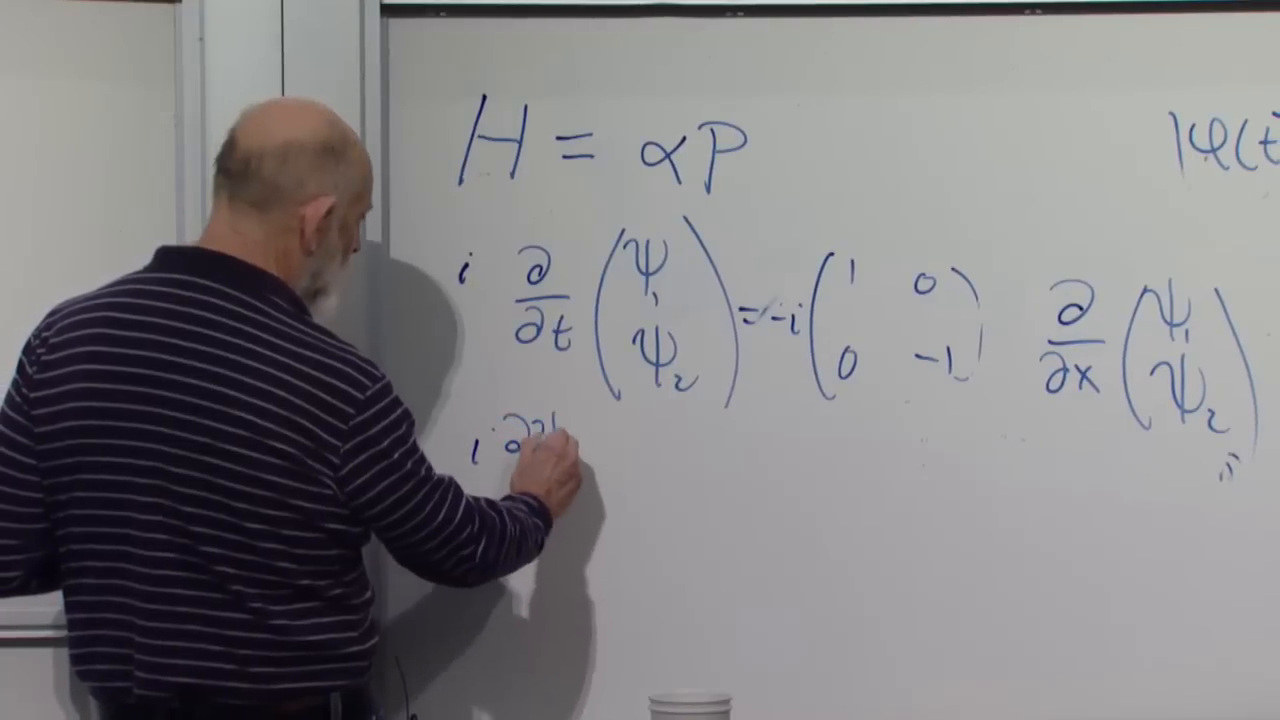
\includegraphics[width=0.94\linewidth]{lecture_09_frame_03.png}
\caption{L’équation sans masse à deux composantes inscrite au tableau : \(H=\alpha P\), où la matrice diagonale attribue des sens de propagation opposés à \(\psi_1\) et à \(\psi_2\).}
\lectureframe{01:26:00}
\end{figure}

Le problème de la propagation dans un seul sens est résolu. Le spectre d’énergie négative demeure, et nous avons découvert un troisième défaut : les deux composantes restent sans masse et se propagent à la vitesse de la lumière. L’étape suivante doit introduire une énergie au repos et coupler les directions.

\section{Ajout de la masse et découverte de l’algèbre de Dirac}

Ajoutons le terme simple le plus général proportionnel à la masse,
\begin{equation}
H=\alpha p+\beta m,
\label{eq:l9-dirac-hamiltonian}
\end{equation}
où \(\beta\) n’agit que sur l’indice des deux composantes. Il aurait pu s’agir de la matrice identité ou d’une autre matrice ; la relation de dispersion relativiste en décidera.

Puisque \(H^2\) doit être égal à \(p^2+m^2\), élevons au carré l’équation~\eqref{eq:l9-dirac-hamiltonian} :
\begin{align}
H^2
&=(\alpha p+\beta m)^2\\
&=\alpha^2p^2+\beta^2m^2
+(\alpha\beta+\beta\alpha)pm.
\label{eq:l9-square-dirac}
\end{align}
Les matrices commutent avec \(p\), car elles agissent sur l’espace interne des deux composantes, tandis que \(p\) agit sur la fonction d’onde spatiale. Pour retrouver l’équation~\eqref{eq:l9-rel-dispersion}, il faut que
\begin{equation}
\alpha^2=\mathbb{1},
\qquad
\beta^2=\mathbb{1},
\qquad
\{\alpha,\beta\}
=\alpha\beta+\beta\alpha=0.
\label{eq:l9-dirac-algebra}
\end{equation}
La première condition est déjà satisfaite par \(\alpha=\sigma_3\). Toute autre matrice de Pauli anticommmute avec elle et a pour carré la matrice identité. Choisissons
\begin{equation}
\beta=
\begin{pmatrix}
0&1\\
1&0
\end{pmatrix}
=\sigma_1.
\label{eq:l9-beta}
\end{equation}
Le choix de \(\sigma_1\) plutôt que de \(\sigma_2\) relève d’une convention de base ; les deux réalisent la même algèbre après un changement de base unitaire.

\begin{classroomqa}
\lecturetimestamp{01:33:00}
\audiencequestion{Dirac a-t-il simplement reconnu que les matrices de Pauli satisfont ces conditions algébriques ?}
\lecturerresponse{La dérivation historique a été menée directement en trois dimensions et a introduit des matrices satisfaisant les relations requises. Une fois les conditions écrites, l’algèbre de Pauli rend immédiate la solution unidimensionnelle : il suffit de choisir deux matrices de Pauli différentes.}
\end{classroomqa}

\begin{classroomqa}
\lecturetimestamp{01:34:24}
\audiencequestion{S’agit-il ici de \(\beta\), le paramètre relativiste de vitesse \(v/c\) ?}
\lecturerresponse{Non. C’est une matrice qui agit sur les composantes du spineur. Cette lettre réutilisée n’est que la notation de Dirac ; elle n’a rien à voir avec la quantité cinématique \(v/c\).}
\end{classroomqa}

En trois dimensions spatiales, les matrices \(2\times2\) ne suffisent pas pour obtenir l’ensemble complet des matrices anticommutantes requises. Cet élargissement sera abordé plus tard. En une dimension, les équations~\eqref{eq:l9-alpha} et \eqref{eq:l9-beta} suffisent.

\section{L’équation de Dirac unidimensionnelle couplée}

En substituant \(p=-i\partial_x\), on obtient l’équation de Dirac unidimensionnelle sous forme hamiltonienne :
\begin{equation}
i\partial_t\Psi
=\left(-i\alpha\partial_x+\beta m\right)\Psi.
\label{eq:l9-one-dimensional-dirac}
\end{equation}
Comme \(\alpha\) est diagonale, son terme dérivé laisse les deux composantes séparées. Comme \(\beta\) est hors diagonale, le terme de masse échange les deux composantes. Écrites composante par composante, les équations sont
\begin{align}
i\partial_t\psi_1
&=-i\partial_x\psi_1+m\psi_2,
\label{eq:l9-dirac-component-one}\\
i\partial_t\psi_2
&=+i\partial_x\psi_2+m\psi_1.
\label{eq:l9-dirac-component-two}
\end{align}

\begin{figure}[htbp]
\centering
\includegraphics[width=0.94\linewidth]{lecture_09_frame_08.png}
\caption{Les équations couplées des composantes inscrites au tableau. Les signes opposés devant les dérivées codent les propagations vers la droite et vers la gauche ; le terme de masse hors diagonale échange \(\psi_1\) et \(\psi_2\).}
\lectureframe{01:37:44}
\end{figure}

Dès que \(m\ne0\), les composantes cessent d’évoluer indépendamment. En élevant au carré l’équation du premier ordre, on retrouve l’opérateur de Klein--Gordon sur chaque composante,
\begin{equation}
\left(\partial_t^2-\partial_x^2+m^2\right)\psi_a=0,
\qquad a=1,2,
\end{equation}
et les ondes planes satisfont \(E^2=p^2+m^2\). Leur vitesse de groupe est
\begin{equation}
v_g=\frac{dE}{dp}=\frac{p}{E},
\end{equation}
et sa valeur absolue est inférieure à un pour toute masse non nulle.

Le lien entre la masse et le mélange des composantes droite et gauche n’est pas fortuit. Un mode se propageant vers la droite et sans masse reste dirigé vers la droite sous toute transformation de Lorentz propre ; aucun observateur subluminal ne peut dépasser la lumière et en inverser le sens. Une particule massive peut être amenée au repos, puis observée dans un référentiel plus rapide se déplaçant dans le même sens, où sa vitesse apparaît inversée. Une théorie relativiste massive ne peut donc pas maintenir les secteurs droit et gauche isolés en permanence. Le terme de masse hors diagonale fournit précisément le couplage nécessaire.

\begin{classroomqa}
\lecturetimestamp{01:40:01}
\audiencequestion{L’échange entre les deux composantes est-il une oscillation chirale ?}
\lecturerresponse{Dans cette base unidimensionnelle, \(\alpha\) distingue les deux directions chirales sans masse. Le terme de masse est hors diagonale et les mélange ; la chiralité n’est donc plus conservée. En ce sens, le terme de masse est à l’origine de l’oscillation chirale.}
\end{classroomqa}

\begin{classroomqa}
\lecturetimestamp{01:40:46}
\audiencequestion{Pourquoi l’équation d’un fermion devrait-elle être la racine carrée de celle d’un boson ?}
\lecturerresponse{Il ne faut pas comprendre les choses ainsi. La relation de dispersion \(E^2=p^2+m^2\) s’applique à toute particule relativiste libre, quelles que soient ses statistiques. L’opérateur de Dirac fournit une factorisation matricielle de l’opérateur de Klein--Gordon, mais cette relation algébrique ne dérive pas les fermions des bosons.}
\end{classroomqa}

\begin{classroomqa}
\lecturetimestamp{01:41:31}
\audiencequestion{Peut-on réduire l’équation à une factorisation scalaire simple en facteurs distincts correspondant aux propagations vers la gauche et vers la droite ?}
\lecturerresponse{Ce n’est que dans la limite sans masse que les deux équations chirales se découplent en facteurs scalaires indépendants. Pour \(m\ne0\), la factorisation utile est matricielle : ce sont les matrices anticommutantes \(\alpha\) et \(\beta\) qui éliminent le terme croisé indésirable.}
\end{classroomqa}

\begin{classroomqa}
\lecturetimestamp{01:42:04}
\audiencequestion{Ces deux équations couplées constituent-elles déjà l’équation de Dirac ?}
\lecturerresponse{Oui. Ensemble, elles forment l’équation de Dirac en une dimension spatiale, écrite de façon équivalente sous la forme compacte de l’équation~\eqref{eq:l9-one-dimensional-dirac}. On peut obtenir une notation covariante plus symétrique en multipliant par \(\beta\), mais cette forme sera présentée plus tard.}
\end{classroomqa}

Deux tâches restent délibérément inachevées. La construction n’a pas éliminé les énergies négatives ; elle a fourni des solutions d’énergie négative dans les deux secteurs directionnels, de sorte que le problème apparaît maintenant plus clairement, et non moins. Et la théorie demeure limitée à une dimension spatiale. L’interprétation des solutions d’énergie négative et l’élargissement de l’algèbre des matrices aux dimensions \(3+1\) sont les prochaines étapes.
